
    1. Функции обработчика прерывания от системного таймера для двух классов ОС: Windows и Unix по литературе на примере защищенного режима:
- по тику;
- по главному тику;
- по кванту
        
    2. Пересчет динамических приоритетов. Динамическими приоритетами являются приоритеты пользовательских процессов. 
В отчете пересчет динамических приоритетов рассматривается отдельно для ОС семейства Windows и для ОС Unix.

\chapter{Функции обработчика прерывания от системного таймера на примере защищенного режима}

\section{Функции обработчика прерывания от системного таймера для ОС семейства UNIX/Linux}

\section{Функции обработчика прерывания от системного таймера для ОС семейства Windows}

\chapter{Пересчет динамических приоритетов}

\section{Пересчет динамических приоритетов для ОС семейства Linux}

\section{Пересчет динамических приоритетов для для ОС семейства Windows}

%\begin{figure}[ph!]
%	\center{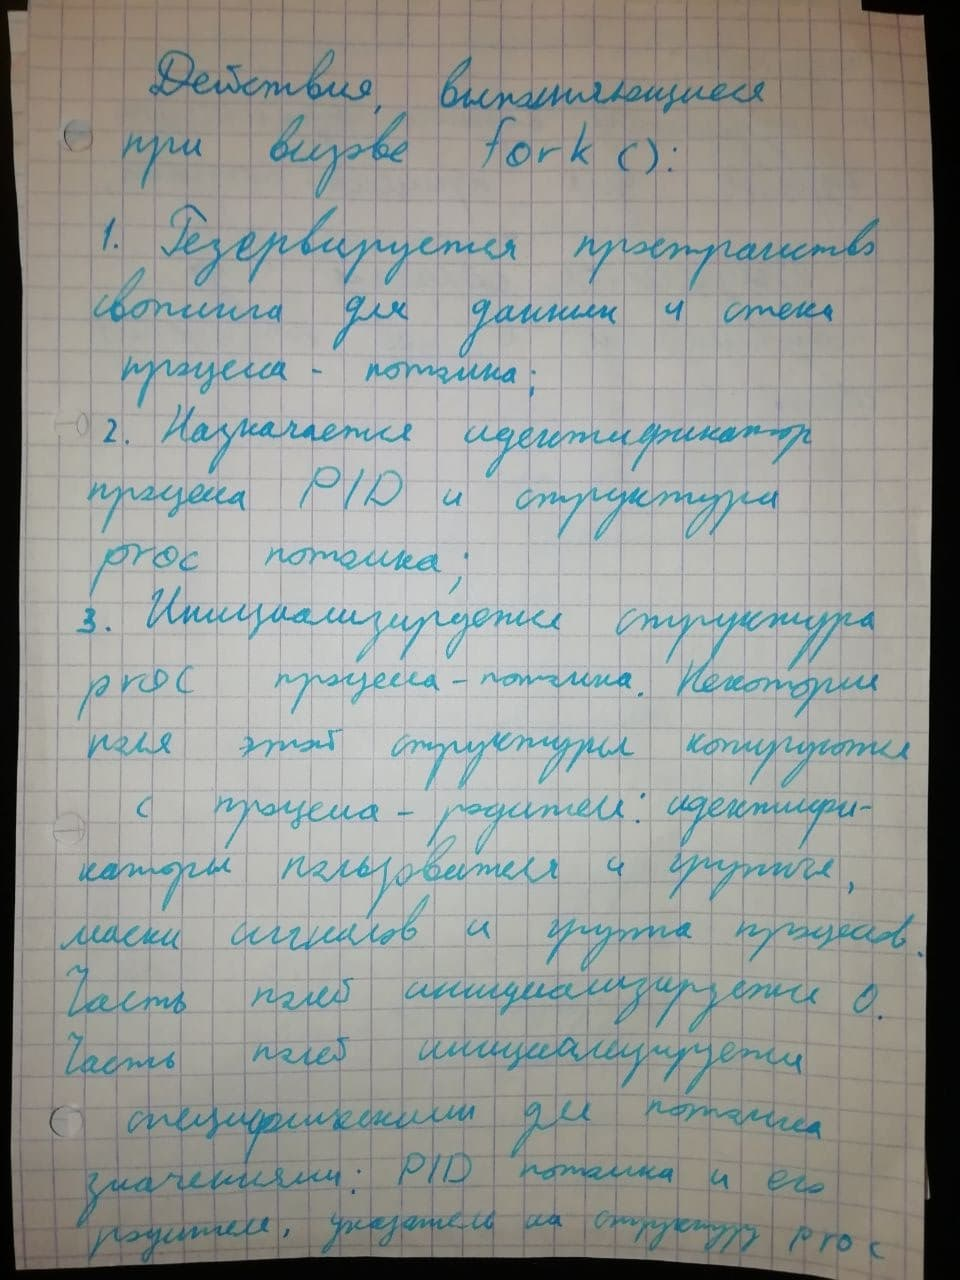
\includegraphics[scale=0.35]{fork_1}}
%	\caption{Конспект fork - часть 1}
%\end{figure}
